\chapter{Disbursement Module: PFE Project}
\label{chap:disbursement_module}

\section{Introduction}
\label{sec:ch5_introduction}

The previous chapters described the platform, its technical base, and the main user flows. This chapter focuses on the academic project assigned during the internship: the Disbursement Module. In Supply Chain Finance, disbursement is not just a button that sends money. It is the controlled execution of a financing decision after an invoice becomes eligible, a program rule is applied, and the bank accepts the payment operation.

The Product Owner refinement sessions clarified the module progressively. Some early assumptions were corrected, and the final business vocabulary became sharper: \texttt{Program}, \texttt{Invoice}, \texttt{Disbursement}, \texttt{FinanceRecord}, and \texttt{Transaction} are distinct concepts. A separate \texttt{FinanceRequest} entity was removed from the model. The \texttt{Disbursement} entity itself carries the information needed to represent the financing request, especially its mode and source.

\section{Context and Motivation}
\label{sec:ch5_context_motivation}

\subsection{Position in the SCF Value Chain}
\label{subsec:ch5_value_chain}

The platform supports invoice financing between a supplier, a buyer, and a bank. A supplier delivers goods or services and issues an invoice. Instead of waiting until maturity, the supplier may receive money earlier. Depending on the program, the financing can be buyer-anchored or supplier-anchored. In a buyer-anchored program, also known as reverse factoring, the buyer's credit profile drives the financing conditions. In a supplier-anchored program, the supplier's credit quality and the buyer's payment history influence the rate and risk model.

The Product Owner also confirmed three request types available on a lodged invoice: early payment, request finance, and request payment. Early payment and request payment do not create a bank disbursement. Request finance does. That boundary matters because the Disbursement Module owns the bank payment execution path, while early payment remains a buyer-supplier settlement flow.

\begin{table}[H]
    \centering
    \caption{Request types available on a lodged invoice}
    \label{tab:ch5_request_types}
    \standardtable
    \begin{tabularx}{\textwidth}{B{0.22\textwidth} Y C{0.20\textwidth} C{0.22\textwidth}}
        \standardtablehead{\textbf{Request type} & \textbf{Parties involved} & \textbf{Bank involved} & \textbf{Invoice final state}}
        Early payment & Buyer and supplier only & No & \texttt{MANUALLY\_PAID} \\
        Request finance & Supplier and bank, with buyer obligation behind the invoice & Yes & \texttt{FINANCED} \\
        Request payment & Buyer pays manually & No & \texttt{MANUALLY\_PAID} \\
    \end{tabularx}
    \standardtableend
\end{table}

\subsection{Architecture Boundary of the Module}
\label{subsec:ch5_architecture_boundary}

The new context confirms that the current SCF backend is a single deployable service organized into internal modules. The Disbursement Module therefore belongs inside \texttt{scf-service}, alongside the Program, Invoice, Finance, Repayment, Counterparty, and Transaction-related modules. The platform still uses Spring Cloud infrastructure around this service: \texttt{adria-gateway}, \texttt{adria-config}, and \texttt{adria-registry}. This choice keeps the product ready for future services without forcing the current business model into unnecessary service splitting.

The module boundary rule is simple: internal modules do not call each other's repositories directly. Cross-module communication must go through service interfaces. For the Disbursement Module, this means invoice eligibility, program configuration, transaction creation, and finance-record creation must be coordinated through application services rather than direct persistence shortcuts.

\subsection{Access Symmetry}
\label{subsec:ch5_access_symmetry}

One Product Owner decision changed the initial understanding of the actors: both buyer and seller can initiate the three request types. In buyer-anchored programs, the supplier may not be a bank client and may not have platform access. In that case, the buyer can act on the supplier's behalf. In supplier-anchored programs, the seller can initiate request payment, receive a payment identifier, and communicate it to the buyer outside the platform.

This access symmetry has design consequences. The module cannot be modeled as a supplier-only flow. It must respect the user's role, program type, and invoice state at the same time.

\section{Requirements and Functional Specification}
\label{sec:ch5_requirements}

\subsection{Functional Requirements}
\label{subsec:ch5_functional_requirements}

The core requirement is to create and execute a disbursement when a financing request is valid. The user can request financing manually, or the system can create an automatic disbursement when the program is configured for it. In both cases, the same eligibility logic protects the bank from financing an invoice outside program limits.

\begin{table}[H]
    \centering
    \caption{Functional requirements of the Disbursement Module}
    \label{tab:ch5_functional_requirements}
    \standardtable
    \begin{tabularx}{\textwidth}{B{0.27\textwidth} Y}
        \standardtablehead{\textbf{Requirement} & \textbf{Description}}
        Manual request finance & Allow a user to select one or more lodged invoices and request financing. \\
        Individual mode & Create one disbursement per selected invoice. A failure on one invoice does not block the others. \\
        Clubbed mode & Create one disbursement for a group of selected invoices and one finance record covering them. \\
        Automatic disbursement & Trigger disbursement automatically when \texttt{program.autoDisbursement = true} and an invoice reaches \texttt{LODGED}. \\
        Eligibility checks & Run the four confirmed checks before any disbursement is created. \\
        Payment gateway submission & Submit the payment request to the external Payment Gateway and store the returned \texttt{paymentRef}. \\
        Async confirmation & Process the Payment Gateway callback through the gateway and Kafka before changing the disbursement state. \\
        Finance record creation & Create the \texttt{FinanceRecord} only when the disbursement reaches \texttt{SUCCESS}. \\
    \end{tabularx}
    \standardtableend
\end{table}

\begin{figure}[H]
    \centering
    
\includegraphics[width=\textwidth, keepaspectratio]{images/ch5_disbursement_use_case.png}
    \caption{Use case diagram of the Disbursement Module}
    \label{fig:ch5_disbursement_use_case}
\end{figure}

\subsection{Eligibility Rules}
\label{subsec:ch5_eligibility_rules}

The eligibility engine runs four checks in sequence. All of them must pass. These checks are not cosmetic validation. They control the bank's exposure to invoice amount, program portfolio cap, requested amount, and tenor.

\begin{table}[H]
    \centering
    \caption{Confirmed eligibility checks}
    \label{tab:ch5_eligibility_checks}
    \standardtable
    \begin{tabularx}{\textwidth}{B{0.14\textwidth} Y B{0.30\textwidth}}
        \standardtablehead{\textbf{Check} & \textbf{Condition} & \textbf{Rejection code}}
        C1 & \texttt{remaining\_eligible\_amount > 0} & \texttt{ELIGIBILITY\_QUOTA\_EXHAUSTED} \\
        C2 & \texttt{program\_disbursement\_count < program.maxDisbursement} & \texttt{PROGRAM\_CAP\_REACHED} \\
        C3 & \texttt{requestedAmount <= remaining\_eligible\_amount} & \texttt{ELIGIBILITY\_AMOUNT\_EXCEEDED} \\
        C4 & \texttt{invoice\_tenor <= program.maxTenorDays} & \texttt{TENOR\_EXCEEDED} \\
    \end{tabularx}
    \standardtableend
\end{table}

The second rule was corrected during refinement. \texttt{maxDisbursement} is not a per-invoice counter. It is a program-level cap. Once the cap is reached, every lodged invoice in the program becomes ineligible until the business defines a later release or override mechanism.

\begin{algorithm}[H]
    \DontPrintSemicolon
    \Data{Program, invoice, requested amount, existing successful disbursements}
    \Result{Eligibility decision and rejection code if any}
    \BlankLine
    Compute \texttt{financed\_amount\_total} for the invoice\;
    Compute \texttt{max\_financeable\_amount = invoice.amount * program.financePercent}\;
    Compute \texttt{remaining\_eligible\_amount}\;
    Count successful disbursements already created under the program\;
    \If{\texttt{remaining\_eligible\_amount <= 0}}{
        Reject with \texttt{ELIGIBILITY\_QUOTA\_EXHAUSTED}\;
    }
    \If{\texttt{program\_disbursement\_count >= program.maxDisbursement}}{
        Reject with \texttt{PROGRAM\_CAP\_REACHED}\;
    }
    \If{\texttt{requestedAmount > remaining\_eligible\_amount}}{
        Reject with \texttt{ELIGIBILITY\_AMOUNT\_EXCEEDED}\;
    }
    \If{\texttt{invoice\_tenor > program.maxTenorDays}}{
        Reject with \texttt{TENOR\_EXCEEDED}\;
    }
    Return eligible\;
    \caption{Disbursement eligibility evaluation}
    \label{alg:ch5_eligibility}
\end{algorithm}

\subsection{Non-functional Requirements}
\label{subsec:ch5_non_functional_requirements}

The module also carries non-functional expectations. Security is handled through Keycloak roles and gateway validation. Payment callback integrity is protected through HMAC signature verification. Traceability is handled through transaction records and state changes. Reliability depends on Kafka because the Payment Gateway confirmation arrives asynchronously and must not be lost if the consumer is temporarily unavailable.

\section{Design}
\label{sec:ch5_design}

\subsection{Domain Model}
\label{subsec:ch5_domain_model}

The confirmed business layer contains five distinct entities. Mixing them would produce a wrong model. A \texttt{Program} governs financing rules. An \texttt{Invoice} is the commercial document. A \texttt{Disbursement} is the payment execution record. A \texttt{FinanceRecord} tracks what the buyer owes the bank after successful disbursement. A \texttt{Transaction} is the business ledger entry visible in inquiry screens.

\begin{table}[H]
    \centering
    \caption{Core entities of the Disbursement Module}
    \label{tab:ch5_core_entities}
    \standardtable
    \begin{tabularx}{\textwidth}{B{0.22\textwidth} Y}
        \standardtablehead{\textbf{Entity} & \textbf{Confirmed role}}
        Program & Central configuration object. Defines program type, finance percentage, maximum disbursement cap, tenor limit, and automatic disbursement flag. \\
        Invoice & Commercial document that becomes financeable when it reaches \texttt{LODGED} and passes eligibility checks. \\
        Disbursement & Payment execution record. Carries \texttt{mode}, \texttt{source}, \texttt{state}, \texttt{amount}, \texttt{paymentRef}, and failure reason. \\
        FinanceRecord & Bank repayment tracker created only after a successful disbursement. It is the handoff artifact to the repayment module. \\
        Transaction & Business ledger entry used by dashboards and transaction inquiry. It records invoice, disbursement, repayment, and early payment movements. \\
    \end{tabularx}
    \standardtableend
\end{table}

\begin{figure}[H]
    \centering
    
\includegraphics[width=\textwidth, keepaspectratio]{images/ch5_disbursement_class_diagram.png}
    \caption{Disbursement domain class diagram}
    \label{fig:ch5_disbursement_class_diagram}
\end{figure}

The following relationship decisions are confirmed:

\begin{itemize}
    \item one \texttt{Program} has one or many \texttt{Invoice} records;
    \item one \texttt{Program} has zero or many \texttt{Disbursement} records;
    \item one \texttt{Disbursement} covers one or many invoices, depending on \texttt{INDIVIDUAL} or \texttt{CLUBBED} mode;
    \item one successful \texttt{Disbursement} creates zero or one \texttt{FinanceRecord};
    \item \texttt{Invoice}, \texttt{Disbursement}, and \texttt{FinanceRecord} generate visible \texttt{Transaction} records.
\end{itemize}

\subsection{Invoice and Disbursement State Machines}
\label{subsec:ch5_state_machines}

The invoice lifecycle uses one main \texttt{status} field. A separate \texttt{invoice\_amount\_state} is used only when the invoice is financed, to distinguish whether the bank is still waiting for repayment or has already been repaid.

\begin{table}[H]
    \centering
    \caption{Disbursement lifecycle states}
    \label{tab:ch5_disbursement_states}
    \standardtable
    \begin{tabularx}{\textwidth}{B{0.27\textwidth} Y}
        \standardtablehead{\textbf{State} & \textbf{Meaning}}
        \texttt{INITIATED} & Disbursement record created and payment submission attempted. A synchronous 422 from the gateway sends it directly to \texttt{FAILED}. \\
        \texttt{PENDING\_CONFIRMATION} & Payment Gateway returned 202 Accepted. The \texttt{paymentRef} is stored while the system waits for async callback. \\
        \texttt{SUCCESS} & Payment Gateway callback confirmed execution. Finance record and transaction effects are triggered. \\
        \texttt{FAILED} & The request failed either immediately or through async callback. The invoice remains \texttt{LODGED} and can be retried. \\
    \end{tabularx}
    \standardtableend
\end{table}

\begin{figure}[H]
    \centering
    
\includegraphics[width=\textwidth, keepaspectratio]{images/ch5_disbursement_state_machine.png}
    \caption{Disbursement lifecycle state machine}
    \label{fig:ch5_disbursement_state_machine}
\end{figure}

\subsection{Manual and Automatic Disbursement}
\label{subsec:ch5_manual_auto_disbursement}

Manual disbursement starts from user action. The user selects one or more lodged invoices, chooses \texttt{INDIVIDUAL} or \texttt{CLUBBED}, and enters the requested amount. The eligibility checks run before the disbursement is created. Figure~\ref{fig:ch5_manual_disbursement_screen} shows the manual disbursement wizard in the platform.

\begin{figure}[H]
    \centering
    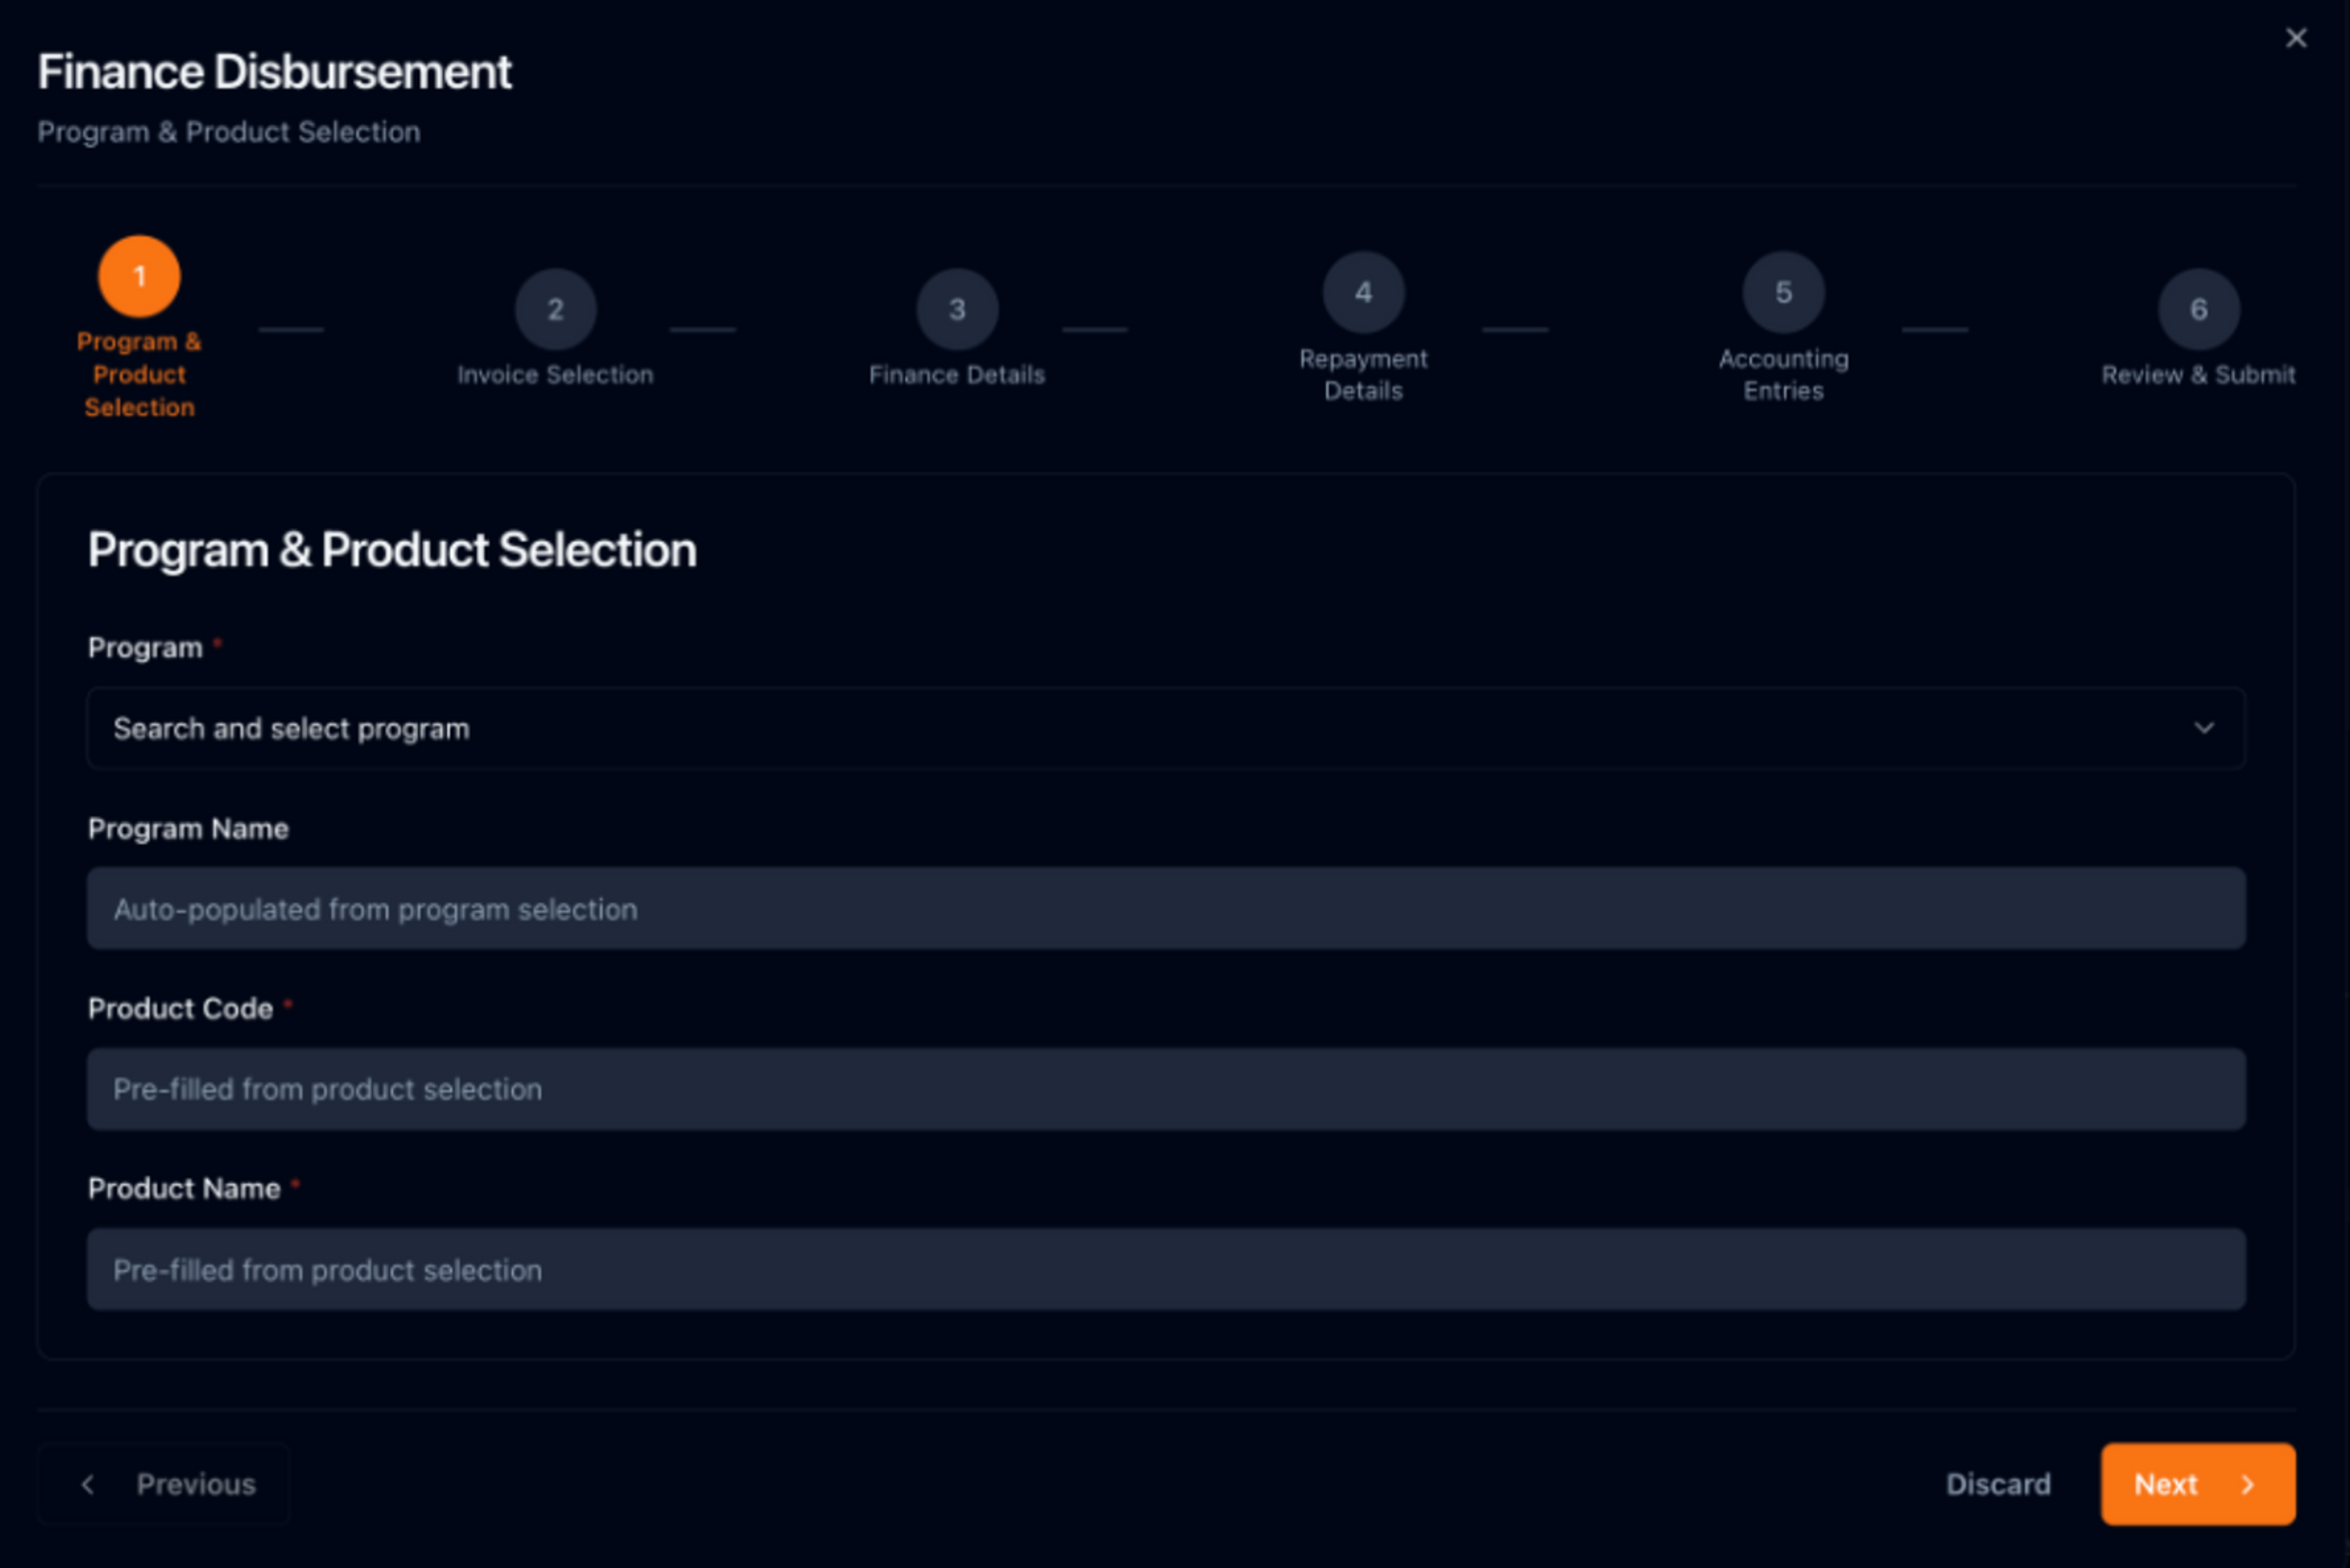
\includegraphics[width=\textwidth, keepaspectratio]{images/platform_manual_disbursement.png}
    \caption{Manual disbursement wizard in the SCF platform}
    \label{fig:ch5_manual_disbursement_screen}
\end{figure}

Automatic disbursement starts without user interaction when \texttt{program.autoDisbursement = true}. This flag represents business pre-approval, not a scheduler by itself. When an invoice reaches \texttt{LODGED}, the invoice module publishes \texttt{invoice.lodged}. The eligibility job consumes the event, runs the same checks, and creates an automatic individual disbursement if the invoice is eligible. In automatic mode, the system always finances 100\% of the remaining eligible amount, and clubbing is not available.

\begin{figure}[H]
    \centering
    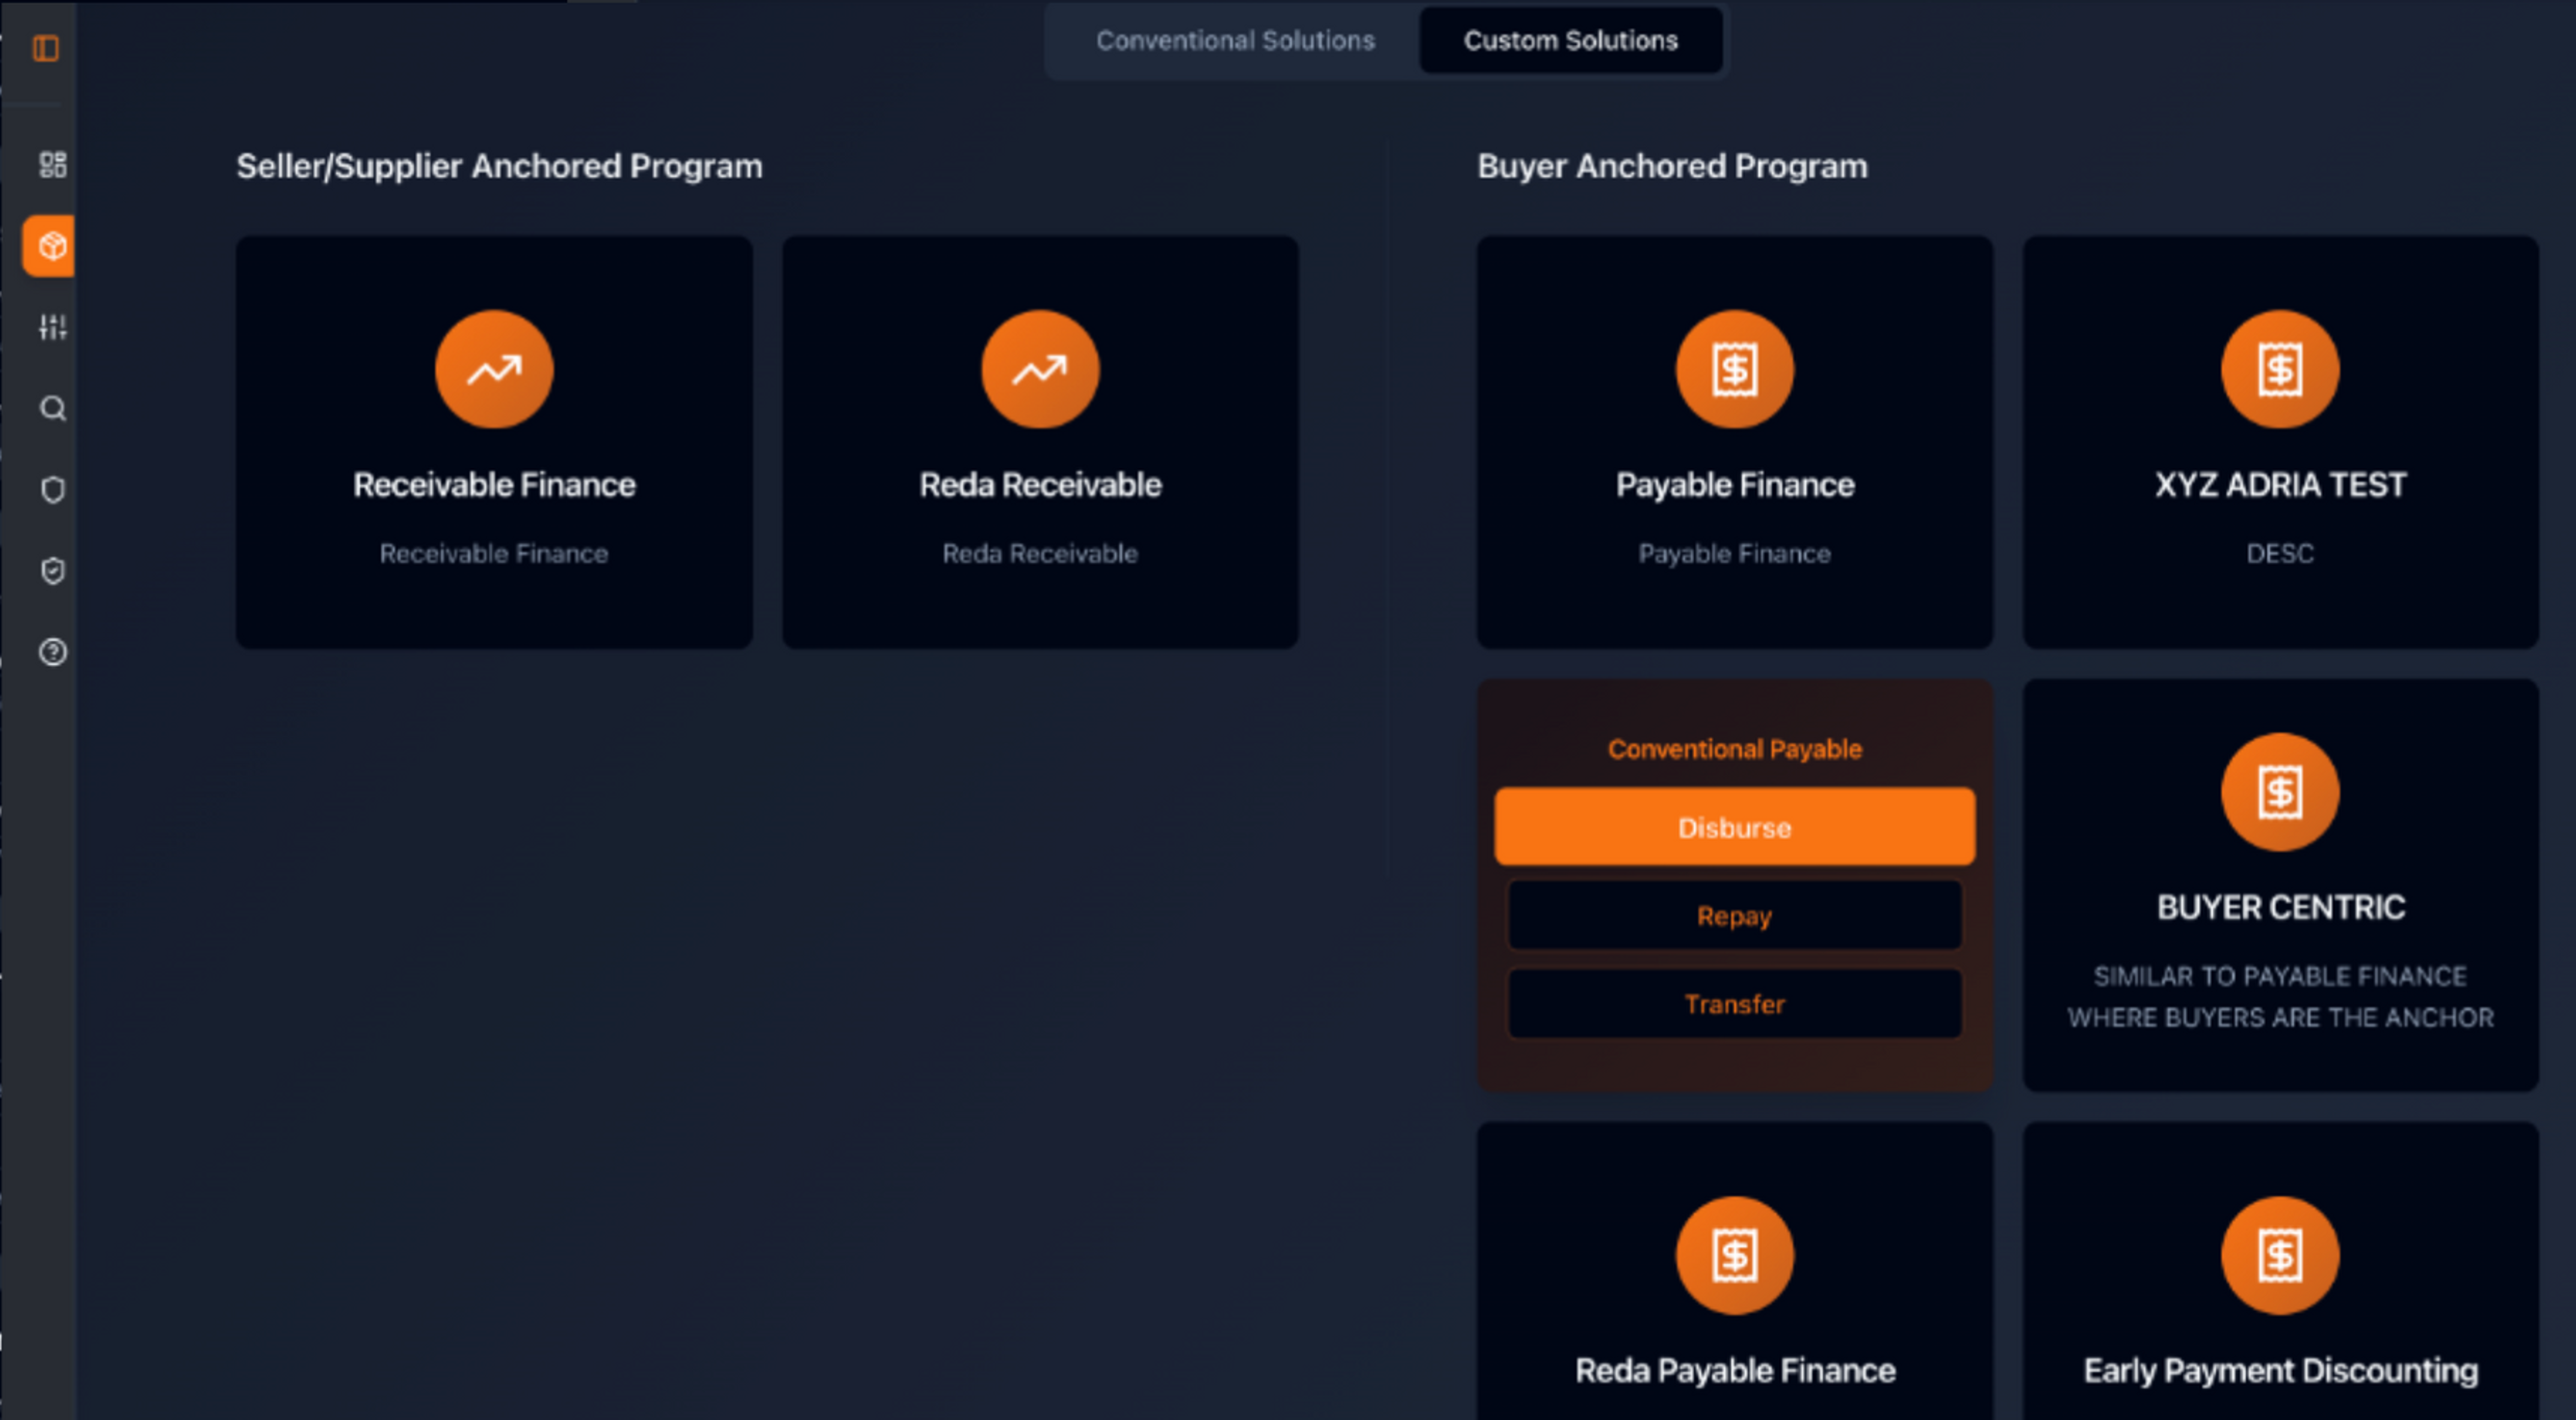
\includegraphics[width=\textwidth, keepaspectratio]{images/platform_auto_disbursement.png}
    \caption{Automatic disbursement entry from the SCF Studio}
    \label{fig:ch5_auto_disbursement_screen}
\end{figure}

\subsection{Payment Gateway Integration}
\label{subsec:ch5_payment_gateway}

The Payment Gateway integration follows a two-phase pattern. During the synchronous phase, the Disbursement service sends an HTTP payment request. A 202 Accepted response means the payment was accepted for processing, not that the money has already moved. The returned \texttt{paymentRef} is stored and used later to match the asynchronous callback.

During the asynchronous phase, the Payment Gateway sends a webhook callback to \texttt{adria-gateway}. The gateway validates the HMAC signature and returns HTTP 200 quickly to avoid external retry storms. It then publishes the callback into Kafka. The \texttt{DisbursementEventConsumer} consumes the event, looks up the disbursement by \texttt{paymentRef}, and applies the final business result.

\begin{figure}[H]
    \centering
    
\includegraphics[width=\textwidth, keepaspectratio]{images/ch5_disbursement_sequence_uml.png}
    \caption{Manual disbursement sequence with Payment Gateway callback and Kafka processing}
    \label{fig:ch5_disbursement_sequence_uml}
\end{figure}

\begin{table}[H]
    \centering
    \caption{Kafka topics related to disbursement and repayment}
    \label{tab:ch5_kafka_topics}
    \standardtable
    \begin{tabularx}{\textwidth}{B{0.25\textwidth} B{0.25\textwidth} Y}
        \standardtablehead{\textbf{Topic} & \textbf{Producer} & \textbf{Purpose}}
        \texttt{invoice.lodged} & Invoice service & Triggers eligibility checking and possible automatic disbursement. \\
        \texttt{invoice.eligible} & Eligibility job & Signals that an invoice can be submitted for payment. \\
        \texttt{payment.callback} & Gateway & Carries Payment Gateway result after HMAC validation. \\
        \texttt{disbursement.success} & Disbursement consumer & Notifies downstream modules that payment was executed. \\
        \texttt{finance.maturity} & Maturity scheduler & Triggers repayment processing at maturity date. \\
    \end{tabularx}
    \standardtableend
\end{table}

\section{Implementation Scope}
\label{sec:ch5_implementation_scope}

\subsection{Frontend Scope}
\label{subsec:ch5_frontend_scope}

The React frontend is in scope for the Disbursement Module. The current platform screen exposes a six-step wizard: program and product selection, invoice selection, finance details, repayment details, accounting entries, and review and submit. This order is important because the repayment schedule is prepared before the user inspects accounting entries and submits the request.

The transaction inquiry page also belongs to the visible scope. It shows invoices in their programs, and it surfaces related finance disbursement and finance repayment transactions when they exist. Finance records are not shown as a separate list; they appear through their transaction records.

\subsection{Backend Scope}
\label{subsec:ch5_backend_scope}

The Disbursement Module owns the flow from invoice lodging up to successful disbursement and FinanceRecord creation. The repayment module is owned separately by another intern and takes over after FinanceRecord creation. The boundary is therefore clean: disbursement creates the handoff artifact; repayment manages maturity, penalties, retries, repayment success, overdue status, and NPA escalation.

\begin{table}[H]
    \centering
    \caption{Scope boundary between Disbursement and Repayment}
    \label{tab:ch5_scope_boundary}
    \standardtable
    \begin{tabularx}{\textwidth}{B{0.28\textwidth} Y}
        \standardtablehead{\textbf{Area} & \textbf{Ownership}}
        Invoice reaches \texttt{LODGED} & Disbursement flow starts from this event. \\
        Eligibility checks & Disbursement Module. \\
        Payment Gateway submission & Disbursement Module. \\
        Payment callback processing & Disbursement Module through gateway and Kafka consumer. \\
        FinanceRecord creation & Disbursement Module creates the handoff artifact after success. \\
        Repayment attempts and overdue handling & Repayment Module. \\
        NPA and crystallization & Repayment Module and later legal/accounting processes. \\
    \end{tabularx}
    \standardtableend
\end{table}

\section{Open Questions and Validation}
\label{sec:ch5_open_questions_validation}

The refinement process also left some questions open. These points should not be resolved by assumption. They need Product Owner confirmation or technical arbitration before implementation is frozen.

\begin{table}[H]
    \centering
    \caption{Open questions identified during refinement}
    \label{tab:ch5_open_questions}
    \standardtable
    \begin{tabularx}{\textwidth}{B{0.28\textwidth} Y}
        \standardtablehead{\textbf{Question} & \textbf{Why it matters}}
        Clubbed partial repayment & If one finance record covers several invoices, partial repayment may require state at the junction-table level. \\
        Exact trigger for \texttt{FINANCED} & The model currently treats FinanceRecord creation as the moment that sets the invoice to \texttt{FINANCED}, but the exact atomic order still needs confirmation. \\
        Portfolio cap UX & When the program cap is reached, all lodged invoices become ineligible. The user-facing notification or queuing behavior is not yet defined. \\
    \end{tabularx}
    \standardtableend
\end{table}

[Insert testing evidence or validation screenshots]

\section{Internship Evaluation and Contribution Summary}
\label{sec:ch5_evaluation_contributions}

The Disbursement Module was prepared while daily work continued inside the Supply Chain Finance Platform Team. This dual rhythm shaped the internship. On one side, sprint tickets required concrete delivery inside the shared codebase. On the other side, the PFE subject required functional analysis, diagrams, refinement with the Product Owner, and a design that could later fit into the platform.

\begin{table}[H]
    \centering
    \caption{Internship timeline and contribution focus}
    \label{tab:ch5_sprint_overview}
    \standardtable
    \begin{tabularx}{\textwidth}{B{0.22\textwidth} Y}
        \standardtablehead{\textbf{Period} & \textbf{Main focus}}
        Weeks 1--2 & Remote onboarding, business training, Java and Spring Boot refresh, and first contact with Adria standards. \\
        Sprint 2 onward & Integration into the SCF team, Jira-based tasks, code review workflow, and platform familiarization. \\
        Middle sprints & Contributions across frontend and backend modules, with regular exposure to SCF entities and user flows. \\
        Sprint gaps and Mondays & Parallel work on the Disbursement Module through Product Owner refinement and diagram validation. \\
        Entering Sprint 8 & Consolidation of platform understanding and preparation of the academic module for future integration. \\
    \end{tabularx}
    \standardtableend
\end{table}

\begin{figure}[H]
    \centering
    
\includegraphics[width=\textwidth, keepaspectratio]{images/ch6_contribution_streams.png}
    \caption{Two contribution streams during the internship}
    \label{fig:ch5_contribution_streams}
\end{figure}

The delivery record contains 20 Jira tickets: 12 related to the SCF service and 8 related to the Foundation Data Library. These tickets produced 40 pull requests in total, covering backend changes, frontend integration work, review adjustments, and supporting corrections. The number is useful because it gives a measurable view of the work, but it should not be read alone. A small validation correction can have more business value than a larger visual change, especially in a banking platform where status transitions and eligibility rules affect risk.

\begin{table}[H]
    \centering
    \caption{Quantitative contribution indicators}
    \label{tab:ch5_quantitative_indicators}
    \standardtable
    \begin{tabularx}{\textwidth}{B{0.30\textwidth} Y}
        \standardtablehead{\textbf{Indicator} & \textbf{Reported value}}
        Jira tickets completed & 20 tickets in total: 12 on the SCF service and 8 on the Foundation Data Library. \\
        Pull requests submitted & 40 pull requests in total. \\
        Work distribution & Each reported ticket involved coordinated backend and frontend work, depending on the module scope. \\
        Main backend areas & SCF service and Foundation Data Library. \\
        Main delivery workflow & Jira ticket, local implementation, Bitbucket pull request, technical lead review, merge, then tester validation. \\
    \end{tabularx}
    \standardtableend
\end{table}

\section{Critical Evaluation and Limitations}
\label{sec:ch5_critical_evaluation}

The strongest part of the internship was the exposure to a real delivery chain. A feature did not end when the code compiled. It had to be pushed, reviewed, corrected when needed, merged, and then checked by testing. That rhythm taught a simple lesson very quickly: professional software is not only about producing code, but about making a change understandable and acceptable to other people.

The work also exposed several difficulties. SCF vocabulary was dense at the beginning, especially around programs, products, invoices, cashflows, disbursement, repayment, and maker/checker governance. The architecture added another layer: gateway routing, JWT validation, shared entity libraries, service boundaries, document storage, and frontend role adaptation all had to be understood before making confident changes.

\begin{table}[H]
    \centering
    \caption{Main difficulties and responses}
    \label{tab:ch5_difficulties}
    \standardtable
    \begin{tabularx}{\textwidth}{B{0.28\textwidth} Y Y}
        \standardtablehead{\textbf{Difficulty} & \textbf{Impact} & \textbf{Response}}
        Banking vocabulary & Domain terms were hard to separate at first, especially when similar concepts appeared in different modules. & Existing modules were studied repeatedly, and Product Owner refinement helped stabilize the vocabulary. \\
        Existing architecture & The platform used several services, shared conventions, and pre-configured Adria standards. & Changes were prepared from existing patterns before adding or modifying behavior. \\
        Maker/checker logic & Governance rules affect visibility, status transitions, approval behavior, and rollback. & The existing approval flows were analyzed before modeling the Disbursement Module. \\
        Role-based frontend behavior & Screens and actions change depending on bank, anchor, or counterparty roles. & Keycloak role extraction and business-view helpers were used as reference points. \\
        Parallel PFE work & The Disbursement Module had to progress before its native integration sprint. & The module was treated as target design, with explicit boundaries and placeholders for final backend validation. \\
    \end{tabularx}
    \standardtableend
\end{table}

The main limitation remains the timing of the Disbursement Module. Since the platform had not yet reached the sprint planned for native integration, the module could not be presented as a completely merged backend feature with final migrations, Swagger contract, and end-to-end evidence. The result is therefore a combination of validated design, visible frontend flow, and future integration preparation.

\section{Skills Acquired and Future Recommendations}
\label{sec:ch5_skills_recommendations}

The internship strengthened both technical and professional skills. On the backend side, it improved practice with Spring Boot services, JPA entities, validation logic, OAuth2 resource-server behavior, and service organization. On the frontend side, it developed stronger habits with React, TypeScript, React Router, React Query, typed service layers, form decomposition, and reusable hooks.

\begin{figure}[H]
    \centering
    
\includegraphics[width=\textwidth, keepaspectratio]{images/ch6_skills_map.png}
    \caption{Main skills acquired during the internship}
    \label{fig:ch5_skills_map}
\end{figure}

The professional side mattered just as much. Jira changed the meaning of a task: it became a visible unit of commitment between developer, reviewer, tester, and team. Pull requests encouraged clearer code and better explanations. Review comments taught precision. Tester feedback taught patience. Product Owner discussions improved the ability to transform business speech into diagrams, statuses, actors, conditions, and system behavior.

\begin{table}[H]
    \centering
    \caption{Skills acquired and reinforced}
    \label{tab:ch5_skills_acquired}
    \standardtable
    \begin{tabularx}{\textwidth}{B{0.25\textwidth} Y}
        \standardtablehead{\textbf{Skill area} & \textbf{Learning outcome}}
        Backend development & Better understanding of Spring Boot services, JPA entities, validation, and governance-oriented design. \\
        Frontend development & Stronger practice with React, TypeScript, form flows, hooks, services, and role-based UI behavior. \\
        Security awareness & Clearer view of OAuth2, Keycloak roles, JWT validation, and protected gateway calls. \\
        Banking domain & Practical understanding of SCF actors, programs, products, invoices, fees, disbursement, and repayment. \\
        Collaboration & Experience with Jira, Bitbucket pull requests, technical lead review, tester validation, and Product Owner refinement. \\
        Technical writing & Ability to transform code, diagrams, and business discussions into an academic report structure. \\
    \end{tabularx}
    \standardtableend
\end{table}

Several recommendations can be drawn from the work. The Disbursement Module should continue toward native integration in the main SCF platform, with a confirmed backend contract, controller endpoints, validation rules, approval lifecycle, and transaction inquiry linkage. Asynchronous processing should also be strengthened for payment callbacks, notification delivery, document processing, and invoice-related events. The platform could later benefit from mobile access for counterparties and richer reporting for bank users who need to monitor financed amounts, overdue repayments, program utilization, counterparty exposure, and approval bottlenecks.

\begin{figure}[H]
    \centering
    
\includegraphics[width=\textwidth, keepaspectratio]{images/ch6_future_roadmap.png}
    \caption{Recommendations for future platform development}
    \label{fig:ch5_future_roadmap}
\end{figure}

\section{Conclusion}
\label{sec:ch5_conclusion}

This chapter presented the Disbursement Module using the clarified context from Product Owner refinement. The module is centered on a precise business act: creating and confirming the bank's payment execution after eligibility checks pass. Its design depends on five distinct entities, a four-check eligibility engine, manual and automatic entry paths, a two-phase Payment Gateway integration, and Kafka-based callback handling.

The chapter also evaluated the internship contribution as a whole. It summarized the delivery rhythm, the reported 20 Jira tickets, the 40 pull requests, the main difficulties encountered, the skills acquired, and the recommendations that can support future development of the platform. This closes the five-chapter body of the report and prepares the transition toward the general conclusion.
